\subsubsection{UC-1 Registrazione}
\begin{itemize}
		\item \textbf{Attori: }Utente non registrato
		\item \textbf{Precondizione: }L'utente ha scelto di registrarsi al sistema.
		\item \textbf{Postcondizione: }Se l'utente è un allievo verrà creato un profilo per esso nel sistema, per un insegnante la richiesta di registrazione verrà segnalata all'amministratore che poi la confermerà.
		\item \textbf{Scenario principale: }
		\begin{enumerate}
		\item L'utente ha scelto di registrarsi al sistema, quindi di creare un nuovo profilo. 
		\item L'utente dovrà scegliere la tipologia di utente, insegnante/allievo. 
		\item L'utente inserirà nome, cognome, username, email e password.
		\item L'utente fornirà il nome della scuola a cui appartiene e la città. 
		\end{enumerate}
		\item \textbf{Estensioni: }
		\begin{itemize}
			\item UC-A Nel caso in cui l'utente tenti l'inserimento di campi non validi vedrà comparire dei messaggi d'errore.
		\end{itemize}
	\end{itemize}
\subsubsection{UC-2 Autenticazione}
		\begin{itemize}
			\item Attori: Attore generico;
			\item Precondizione: l'utente si trova nella vista principale dell'applicazione;
			\item Postcondizione: l'utente ha eseguito l'accesso con il ruolo di allievo o insegnante.
			\item Scenario principale:
				\begin{enumerate}
					\item l'utente accede all'area di autenticazione;
					\item l'utente inserisce la propria email e password;
				\end{enumerate}
				\item Estensioni:
				\begin{itemize}
					\item UC-X Nel caso in cui l'utente tenti l'inserimento di campi non validi vedrà comparire messaggi d'errore.
				\end{itemize}
		\end{itemize}
		
	\subsubsection{UC-3 Modifica profilo}
		\begin{itemize}
			\item Attori: Insegnante, allievo;
			\item Precondizione: l'utente si trova nella vista principale dell'applicazione;
			\item Postcondizione: l'utente ha modificato i propri dati personali.
			\item Scenario principale:
				\begin{enumerate}
					\item l'utente accede all'area del proprio profilo;
					\item l'utente modifica username, password, scuola, città;
				\end{enumerate}
				\item Estensioni:
				\begin{itemize}
					\item UC-X Nel caso in cui l'utente tenti l'inserimento di campi non validi vedrà comparire messaggi d'errore.
				\end{itemize}
		\end{itemize}
		
	\subsubsection{UC-4 Conferma richiesta insegnante}
		\begin{itemize}
			\item Attori: Amministratore;
			\item Precondizione: l'amministratore si trova nella vista principale dell'applicazione;
			\item Postcondizione: l'amministratore ha confermato l'utente richiedente il ruolo di insegnante.
			\item Scenario principale:
				\begin{enumerate}
					\item l'amministratore visualizza la lista degli utenti che richiedono il ruolo di insegnante;
					\item l'amministrazione selezione l'utente da confermare;
				\end{enumerate}
		\end{itemize}
					
	\subsubsection{UC-5 Rifiuto richiesta insegnante}
		\begin{itemize}
			\item Attori: Amministratore;
			\item Precondizione: l'amministratore si trova nella vista principale dell'applicazione;
			\item Postcondizione: l'amministratore ha rifiutato l'utente richiedente il ruolo di insegnante.
			\item Scenario principale:
				\begin{enumerate}
					\item l'amministratore visualizza la lista degli utenti che richiedono il ruolo di insegnante;
					\item l'amministrazione selezione l'utente da rifiutare;
				\end{enumerate}
		\end{itemize}

\subsubsection{UC-6 Errore campi non validi o mancanti}
\begin{itemize}
\item \textbf{Attori: } utente generico
\item \textbf{Precondizione: }L'utente ha inserito dei campi non validi.
\item \textbf{Postcondizione: }Il sistema mostra un messaggio d'errore per spronare l'utente a ricontrollare i campi non validi.
\item \textbf{Scenario principale: }
		\begin{enumerate}
		\item L'utente ha provato a inserire dei campi non validi.
		\item All'utente viene mostrato un messaggio d'errore che invita a ricontrollare i campi non validi.
		\end{enumerate}.
\end{itemize}
\subsubsection{UC-7 Ricerca esercizi disponibili}
		\begin{itemize}
			\item Attori: allievo, insegnante;
			\item Precondizione: l'utente si trova nella vista principale dell'applicazione;
			\item Postcondizione: l'utente ottiene una lista degli esercizi filtrati.
			\item Scenario principale:
				\begin{enumerate}
					\item l'utente accede all'area dedicata alla ricerca degli esercizi;
					\item l'utente può filtrare l'esercizio in base al suo nome;
					\item l'utente può filtrare l'esercizio in base alla frase;
					\item l'utente può filtrare l'esercizio in base all'autore;
					\item l'utente può filtrare l'esercizio in base agli argomenti trattati;
				\end{enumerate}
			\item Estensioni:
				\begin{itemize}
					\item UC-7.1 Nel caso in cui l'utente tenti l'inserimento di campi non validi vedrà comparire messaggi d'errore.
				\end{itemize}
		\end{itemize}
\subsubsection{UC-7.1 Nessun esercizio compatibile con i filtri}
\begin{itemize}
		\item \textbf{Attori: } Insegnante, Allievo
		
		\item \textbf{Precondizione: }L'utente ha impostato i filtri per la ricerca, ma questi limitano la ricerca a tal punto da non essere compatibili con nessun esercizio pubblicato nella piattaforma.
		\item \textbf{Postcondizione: }L'utente visualizza un messaggio d'errore che lo invita a modificare i valori impostati nei filtri di ricerca.
		\item \textbf{Scenario principale: }
		\begin{enumerate}
		\item L'utente non ha impostato i filtri correttamente.
		 \item L'utente visualizza un messaggio d'errore che lo invita a modificare i valori impostati nei filtri di ricerca.
		\end{enumerate}
\end{itemize}
\subsubsection{UC-8 Frase già esistente}
\begin{itemize}
\item \textbf{Attori: }Insegnante, Allievo

\item \textbf{Precondizione: }L'utente ha inserito una frase che è già esistente nel sistema.
\item \textbf{Postcondizione: }Verrà mostrato un messaggio per notificare l'evento all'utente.
\item \textbf{Scenario principale: }
		\begin{enumerate}
		\item L'utente ha inserito una frase.
		\item Questa risulta essere già nella piattaforma.
		\item L'utente verrà visualizzerò un messaggio di notifica dell'evento.
		\end{enumerate}
\end{itemize}

					
\subsection{Attore Insegnante}
\subsubsection{UC-9 Modifica esercizio}
\begin{itemize}
		\item \textbf{Attori: }Insegnante
		\item \textbf{Precondizione: }L'insegnate ha selezionato l'esercizio da modificare.
		\item \textbf{Postcondizione: }L'utente ha modificato l'esercizio se non era lui l'autore l'esercizio viene aggiunto alla lista dei suoi esercizi. 
		\item \textbf{Scenario principale: }
		\begin{enumerate}
		\item L'utente ha scelto un esercizio, questo può essere risultato di una ricerca, oppure selezionato dalla lista di esercizi inseriti dall'insegnante. 
		\item L'utente può modificare il nome dell'esercizio. 
		\item L'utente può modificare la frase dell'esercizio. 
		\item L'utente può modificare gli argomenti trattati dall'esercizio.
		\item L'utente può modificare una soluzione vedi UC-14.
		\item L'utente può eliminare una soluzione vedi UC-11.
		\item L'utente può aggiungere una soluzione vedi UC-13.
		\end{enumerate}
		\item \textbf{Estensioni: }
		\begin{itemize}
			\item UC-A Nel caso in cui l'utente tenti l'inserimento di campi non validi vedrà comparire dei messaggi d'errore.
		\end{itemize}
	\end{itemize}
\subsubsection{UC-10 Visualizzazione esercizi inseriti}
\begin{itemize}
\item \textbf{Attori: }Insegnante
		\item \textbf{Precondizione: }L'insegnate si trova nell'area del suo profilo e ha scelto di visualizzare tutti gli esercizi da lui inseriti.
		\item \textbf{Postcondizione: }L'insegnante visualizza una lista di esercizi inseriti. 
		\item \textbf{Scenario principale: }
		\begin{enumerate}
		\item L'insegnante vede una lista di esercizi che lui stesso ha inserito nella piattaforma.
		\item L'insegnante può eliminare uno o più esercizi.
		\item L'insegnante può modificare un esercizio vedi UC-9.
		\end{enumerate}
	\end{itemize}
\subsubsection{UC-11 Eliminare una soluzione di un esercizio}
\begin{itemize}
\item \textbf{Attori: }Insegnante
		\item \textbf{Precondizione: }L'insegnate ha selezionato la soluzione da eliminare.
		\item \textbf{Postcondizione: }La soluzione selezionata viene eliminata. 
		\item \textbf{Scenario principale: }
		\begin{enumerate}
		\item L'utente sceglie una soluziona da eliminare.
		\item La soluzione scelta viene eliminata.
		\end{enumerate}
	\end{itemize}

\subsubsection{UC-12 Inserimento esercizio}
\begin{figure}[htbp]
	\centering
	%inserire immagine diagramma
	\caption{UC-1 Inserimento esercizio}
\end{figure}
	\begin{itemize}
		\item \textbf{Attori: }Insegnante
		\item \textbf{Precondizione: }L'utente si è loggato come insegnante ed ha scelto di inserire un nuovo esercizio.
		\item \textbf{Postcondizione: }Il sistema salverà l'esercizio, esso verrà aggiunto alla lista degli esercizi creati dall'insegnante
		\item \textbf{Scenario principale: }
		\begin{enumerate}
		\item L'utente si è loggato come insegnante e ha scelto di inserire un nuovo esercizio. 
		\item Fornisce un nome dell'esercizio. 
		\item Successivamente inserirà una frase vedi UC-13, la richiesta dell'esercizio è compiere l'analisi grammaticale di questa frase. 
		
		\item Poi inserirà gli argomenti. 
		\item L'utente sceglierà se l'esercizio inserito dovrà essere pubblico o privato.
		\item Infine l'esercizio potrà essere salvato.
		\end{enumerate}
		
		\item \textbf{Estensioni: }
		\begin{itemize}
		\item UC-12.1.1 Nel caso in cui il nome inserito sia già esistente tra gli esercizi creati.
		\item UC-C La frase potrebbe essere già presente nella piattaforma.
		\item UC-13.3.1 Se la frase fosse già presente nella piattaforma, durante la fase di inserimento della soluzione l'utente potrà scegliere di utilizzare la soluzione della frase già esistente, altrimenti verrà proposta una soluzione generata automaticamente.
		\item UC-A I campi compilati potrebbero presentare errori. In questo caso il salvataggio non verrà eseguito e un messaggio d'errore segnalerà all'utente di ricontrollare i campi non validi.
		\end{itemize}
	\end{itemize}
\subsubsection{UC-12.1 Inserimento nome esercizio}
\begin{itemize}
\item \textbf{Attori: }Insegnante

\item \textbf{Precondizione: }Insegnante ha scelto di inserire un nuovo esercizio e il sistema attende che l'utente inserisca un nome per questo esercizio
\item \textbf{Postcondizione: }La casella contenente il nome dell'esercizio che l'utente vuole inserire è compilata, e se il nome inserito risulterà corretto in fase di salvataggio non verranno riscontrati problemi.
\item \textbf{Scenario principale: }
		\begin{enumerate}
		\item L'insegnante, volendo inserire un nuovo esercizio, inserisce un nome per tale esercizio.
		\end{enumerate}
		
\end{itemize}
\subsubsection{UC-12.1.1 Errore nome già esistente}
\begin{itemize}
\item \textbf{Attori: }Insegnante

\item \textbf{Precondizione: }Insegnante ha inserito un nome per l'esercizio, ma il nome risultà essere già presente tra gli esrcizi creati dall'insegnante.
\item \textbf{Postcondizione: }Verrà mostrato un messaggio d'errore che riferirà all'utente di modificare il nome inserito.
\item \textbf{Scenario principale: }
		\begin{enumerate}
		\item L'insegnante ha inserito un nome per l'esercizio.
		\item Il nome inserito è già presente tra gli esercizi creati dall'insegnante.
		\item L'insegnante visualizza un messaggio d'errore che riferirà di modificare i dati inseriti.
		\end{enumerate}
		
\end{itemize}
\subsubsection{UC-12.2 Inserimento frase}
\begin{itemize}
\item \textbf{Attori: }Insegnante

\item \textbf{Precondizione: }L'insegnante ha scelto di inserire un nuovo esercizio e il sistema attende che l'utente inserisca una frase per questo esercizio.
\item \textbf{Postcondizione: }La casella per l'inserimento della frase dell'esercizio è compilata, e se la frase inserita risulterà valida in fase di salvataggio non verranno riscontrati problemi.
\item \textbf{Scenario principale: }
		\begin{enumerate}
		\item L'insegnante inserisce una frase per tale esercizio.
		\end{enumerate}
\end{itemize}

\subsubsection{UC-13 Aggiunta di una soluzione}
\begin{figure}[htbp]
	\centering
	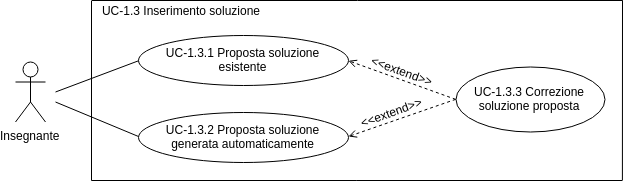
\includegraphics[scale=0.7]{images/UC-1_3.png}
	\caption{UC-1.3 Inserimento soluzione}
\end{figure}
\begin{itemize}
\item \textbf{Attori: }Insegnante

\item \textbf{Precondizione: }L'insegnante ha inserito una frase, ora può scegliere tra una proposta di soluzione esistente e una proposta di soluzione generata automaticamente, nel caso la frase inserita sia già esistente nel sistema. Altrimenti verrà proposta solo la soluzione generata automaticamente.
\item \textbf{Postcondizione: }L'utente ha scelto tra la soluzione già esistente e quella generata automaticamente. Sceglierà poi se aggiungere la soluzione proposta o modificarla.
\item \textbf{Scenario principale: }
		\begin{enumerate}
		\item L'insegnante vuole aggiungere una soluzione per l'esercizio. 
		\item Nel caso esista già una soluzione per tale frase l'utente può scegliere di partire dalla la soluzione già esistente nella piattaforma.
		\item Altrimenti può sempre scegliere di partire da una soluzione generata automaticamente. 
		\item L'utente aggiunge la soluzione proposta oppura sceglie di modificarla. 
		\item Viene chiesto all'utente se vuole aggiungere un'altra soluzione all'esercizio, in 
		caso affermativo l'utente ripartirà dal UC-13
		\end{enumerate}	
\item \textbf{Estensioni: }
		\begin{itemize}
		\item UC-14 L'utente potrà correggere la soluzione proposta se questa non dovesse soddisfarlo.
		\end{itemize}
\end{itemize}


\subsubsection{UC-14 Modifica soluzione}
\begin{itemize}
\item \textbf{Attori: }Insegnante

\item \textbf{Precondizione: }L'insegnante ha scelto di modificare la soluzione.
\item \textbf{Postcondizione: }La soluzione per la frase inserita è stata modicifcata e risulta essere compilata.
\item \textbf{Scenario principale: }
		\begin{enumerate}
		\item L'insegnante modifica una soluzione esistente oppure corregge eventuali errori di una soluzione proposta. 
		\item Viene chiesto all'utente se vuole aggiungere un'altra soluzione all'esercizio, in 
		caso affermativo viene aggiunta la soluzione appena corretta e l'utente ripartirà dal UCX-1.3
		\end{enumerate}
\end{itemize}

\subsubsection{UC-12.3 Inserimento argomenti}
\begin{itemize}
\item \textbf{Attori: }Insegnante

\item \textbf{Precondizione: L'insegnante sta inserendo un esercizio, gli viene richiesta la compilazione di una lista di argomenti presenti nell'esercizio}
\item \textbf{Postcondizione: L'insegnante ha selazionato gli argomenti trattati nell'esercizio.}
\item \textbf{Scenario principale: }
		\begin{enumerate}
		\item L'insegnante sta inserendo un esercizio. 
		\item L'insegnante seleziona gli argomenti che vengono toccati nell'esercizio. 
		\end{enumerate}
\end{itemize}
\subsubsection{UC-12.4 Scelta esercizio pubblico o privato}
\begin{itemize}
\item \textbf{Attori: }Insegnante

\item \textbf{Precondizione: }L'insegnante deve scegliere la modalità di pubblicazione dell'esercizio nella piattaforma. Ad esso vengono proposte due modalità di salvataggio: pubblico o privato.
\item \textbf{Postcondizione: }La scelta, pubblico o privato, viene selezionata.
\item \textbf{Scenario principale: }
		\begin{enumerate}
		\item L'utente vuole salvare l'esercizio inserito.
		\item L'utente sceglie la modalità di pubblicazione dell'esercizio nella piattaforma. 
		\item Può scegliere la modalità pubblico cioè visibile a tutti gli altri insegnanti e allievi della piattaforma.
		\item Oppure la modalità privato, ovvero l'esercizio viene salvato unicamente nella lista di esercizi dell'utente ma non è visibile ad altri insegnanti o ad altri allievi registrati.
		\end{enumerate}
\end{itemize}

\newpage


					
					
					
\subsection{Attore Allievo}
	

	\subsubsection{UC-15 Esecuzione esercizio}
		\begin{itemize}
			\item Attori: Allievo
			\item Precondizione: l'allievo ha selezionato un esercizio da eseguire;
			\item Postcondizione: l'allievo ha terminato i quesiti proposti dell'esercizio.
			\item Scenario principale:
				\begin{enumerate}
					\item l'allievo sceglie la classe grammaticale per ogni parola presentata.
				\end{enumerate}
			\item Estensioni: 
				\begin{itemize}
					\item UC-6 Nel caso in cui l'utente tenti l'inserimento di campi non validi vedrà comparire messaggi d'errore.
				\end{itemize}
			\item Inclusioni:
				\begin{itemize}
					\item UC-16 Nel caso in cui l'esercizio sia terminato;
				\end{itemize}
			\end{itemize}

	\subsubsection{UC-16 Valutazione esercizio}
	\begin{itemize}
			\item Attori: Allievo
			\item Precondizione: L'allievo ha completato l'esecuzione dell'esercizio;
			\item Postcondizione: L'allievo visualizza la valutazione dell'esercizio.
			\item Scenario principale:
				\begin{enumerate}
					\item l'allievo al termine dell'esecuzione dell'esercizio riceve la valutazione.
				\end{enumerate}
			\end{itemize}
			
	\subsubsection{UC-17 Visualizzazione progressi}
	\begin{itemize}
			\item Attori: Allievo
			\item Precondizione: L'allievo si trova nella vista principale dell'applicazione;
			\item Postcondizione: L'allievo visualizza i progressi svolti fino a quel momento.
			\item Scenario principale:
				\begin{enumerate}
					\item l'allievo prima e/o dopo l'esecuzione di uno o più esercizi può visualizzare i progressi raggiunti.
				\end{enumerate}
			\end{itemize}

